\documentclass[12pt]{article}
\usepackage{amsmath}
\usepackage{fancyhdr}
\usepackage{geometry}
\usepackage{parskip}
\usepackage{pdfpages}
\usepackage{graphicx}
\graphicspath{{./}}
\geometry{letterpaper, portrait, margin=1in}
\setlength{\parindent}{0pt}

\title{Math 252 Homework\\
\large Sections 5.1 \& 5.2}
\date{2016/04/24}
\author{Solomon Greenberg}

\fancyhf{}
\pagestyle{fancy}

\lhead{Math 252 Homework --- Section 5.1 \& 5.2}
\rhead{Solomon Greenberg}



\begin{document}
    \pagenumbering{gobble}
    \newpage
    \pagenumbering{arabic}
    \paragraph*{5.1:} 1, 3, 5, 11, 12, 13, 15, 17, 19
    \paragraph*{5.2:} 1, 3, 5, 7, 9, 10, 12, 17, 19, 22, 31, 32, 35, 39, 31, 43

    \section*{Chapter 5.1}
    \paragraph*{1:\\} 
    4 rectangles:\\
        Lower estimate: left to right rectangles:\\
            Heights: ${2, 2.75, 5, 5.75}$\\
            Area: $2*2 + 2.75*2 + 5*2 + 5.75*2 = 31$\\
        Upper estimate: right to left rectangles\\
            Heights: ${8, 5.75, 5, 2.75}$\\
            Area: $2*8 + 2*5.75 + 2*5 + 2*2.75 = 43$\\
    8:
        Lower:
            Heights: ${2, 3, 3.75, 4.5, 5, 5.75, 5.5, 5.9, 6}$\\
            Area: $41.4$\\
        Upper:
            Heights: ${6, 5.9, 5.5, 5.75, 5, 4.5, 3.75, 3}$\\
            Area: $45.4$\\
    
    \paragraph*{3:\\}
    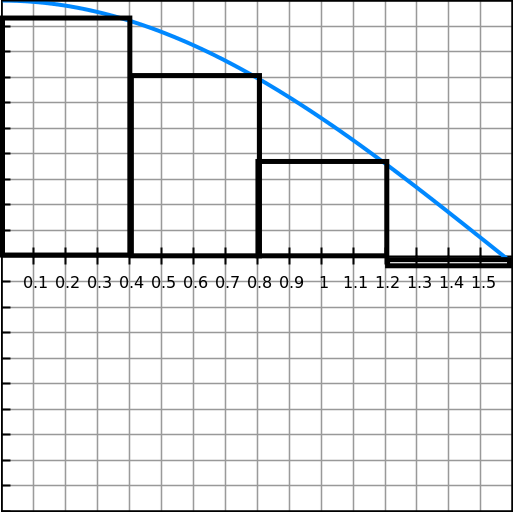
\includegraphics[scale=.333]{3.png}\\\\
    a: Area $ = 0.55$\\
    b: Area $ = 1.55$\\
    
    \paragraph*{5:\\}
    $f(x) = 1 + x^2, [-1, 2]$\\
    a: $\Delta x \sum\limits_{j=1}^{N}f(a + j \Delta x) = 8$\\
    b: $\Delta x \sum\limits_{j=0}^{N-1}f(a + j \Delta x) = 5$\\
    c: $\Delta x \sum\limits_{j=1}^{N}f(a + (j-\frac{1}{2}) \Delta x) = 5.75$\\
    Midpoint (c) seems to be the most accurate.

    \paragraph*{11:\\}
    Lower: $11.5667$\\
    Upper: $14.9333$\\

    \paragraph*{12:\\}
    a. $25.8$\\
    b. $25.2$\\
    c. Yes. The second is the upper estimate and the first the lower.

    \paragraph*{13:\\}
    Lower: 7\\
    Upper: 6.32\\

    \paragraph*{15:\\}
    Left endpoint: $\frac{70}{6} + \frac{50}{6} + \frac{35}{6} + \frac{25}{6} + \frac{15}{6} + \frac{10}{6} = 34.1667$\\
    Right endpoint: $\frac{50}{6} + \frac{35}{6} + \frac{25}{6} + \frac{15}{6} + \frac{10}{6} + \frac{0}{6} = 22.5$\\
    Avg: $28.333$\\

    \paragraph*{17:\\}
    $\Delta x = \frac{3-1}{N} = \frac{2}{N}$\\
    $f(x) = \frac{2x}{x^2 + 1}$\\
    $\lim_{N \to \infty} \Delta x \sum\limits_{j=1}^{N}f(1 + j \Delta x)$\\

    \paragraph*{19:\\}
    $\Delta x = \frac{0-\pi/2}{N} = \frac{-\pi/2}{N}$\\
    $f(x) = x \cdot \cos(x)$ \\
    $\lim_{N \to \infty} \Delta x \sum\limits_{j=1}^{N}f(1 + j \Delta x)$\\


\thispagestyle{fancy}

\end{document}

